\section{Graph Algorithms}

Uniformed search ya da blind search, problemin çözümüne dair hiçbir ön bilgi (heuristic) kullanmadan yalnızca mevcut kuralları takip ederek çözüm bulmaya çalışan algoritmalardır. Yani arama sırasında, hangi düğümün daha avantajlı olabileceğine dair ekstra bir bilgi yoktur, her düğüm eşit derecede değerlendirilir. Herhangi bir maliyet fonksiyonu ya da hedefe yaklaşmayı belirten bir strateji kullanmazlar. 

\begin{itemize}
    \item Breath-First Search (BFS)
    \item Depth-First Search (DFS)
    \item Uniform Cost Search (UCS)
    \item Depth-Limited Search
    \item Iterative Deepening Depth First Search
    \item Bidirectional Search
\end{itemize}

Informed search ya da heuristic (sezgisel) arama, problemin çözümüne dair önceden bilgi kullanarak (heuristic fonksiyonu) aramayı hızlandıran algoritmalardır. Bu algoritmalar, hangi düğümlerin hedefe daha yakın olduğunu tahmin etmek için bir değerlendirme fonksiyonu kullanırlar. Böylece arama daha verimli hale gelir. Bunlar:

\begin{itemize}
    \item Best First Search
    \item A* Search
\end{itemize}

\subsubsection{Traversal Algoritmhs}

\begin{itemize}
    \item Breath-First Search (BFS)
    \item Depth-First Search (DFS)
\end{itemize}

\subsubsection{Shortest Path Algoritmhs}

\begin{itemize}
    \item Dijsktra's Algorithm
    \item Bellman-Ford Algorithm
    \item Floyd-Warshall Algorithm
    \item A* Algorithm
\end{itemize}

\subsubsection{Minimum Spanning Tree (MST) Algoritmhs}

\begin{itemize}
    \item Kruskal's Algorithm
    \item Prim's Algorithm
    \item Boruvka's Algorithm
\end{itemize}

\subsubsection{Topological Sorting}

\begin{itemize}
    \item Kahn's Algorithm
    \item DFS-based Topological Sort
\end{itemize}

\subsubsection{Connected Components Algoritmhs}

\begin{itemize}
    \item Union-Find Algorithm
    \item Kosaraju's Algorithm
    \item Tarjan's Algorithm
\end{itemize}

\subsubsection{Maximum Flow Algoritmhs}

\begin{itemize}
    \item Ford-Fulkerson Algorithm
    \item Edmonds-Karp Algorithm
    \item Dinic's Algorithm
    \item Push-Relabel Algorithm
\end{itemize}

\subsubsection{Graph Coloring Algorithms}

\begin{itemize}
    \item Greedy Coloring Algorithm
    \item Backtracking-based Coloring
    \item Weish-Powell Algorithm
    \item Matching Algorithms
\end{itemize}

\newpage

\subsection{Breath-First Search (BFS)}

Breadth-First Search (BFS), bir graf veya ağaç üzerindeki düğümleri katman katman ziyaret eden bir arama algoritmasıdır. BFS, genişlik öncelikli arama yaparak önce bir düğümün tüm komşularını ziyaret eder, ardından bir sonraki seviyedeki komşulara geçer. Yani, bir düğümden mümkün olan en kısa yolda ulaşabileceğimiz tüm düğümleri ziyaret ettikten sonra daha derindeki düğümlere gider. BFS önce kök düğümü (başlangıç noktası) ziyaret eder ve sonra bu düğüme komşu olan düğümleri keşfeder. Sonrasında bu komşuların komşuları ziyaret edilir. Eğer her kenarın ağırlığı eşit ise, BFS algoritması başlangıç noktasından diğer düğümlere olan en kısa yolu bulur. Eğer bir çözüm varsa, BFS onu mutlaka bulur. Eğer her kenar aynı ağırlıktaysa (ağırlıksız grafiklerde), BFS optimal çözümdür, yani en kısa yolu bulur. Graf, $V$ düğüm ve $E$ kenardan oluşuyorsa, zaman karmaşıklığı $O(V + E)$'dir. Yani her düğüm bir kez ziyaret edilir ve her kenar bir kez işlenir.

\subsubsection{Python Kodu}

\begin{figure}[h]
    \centering
    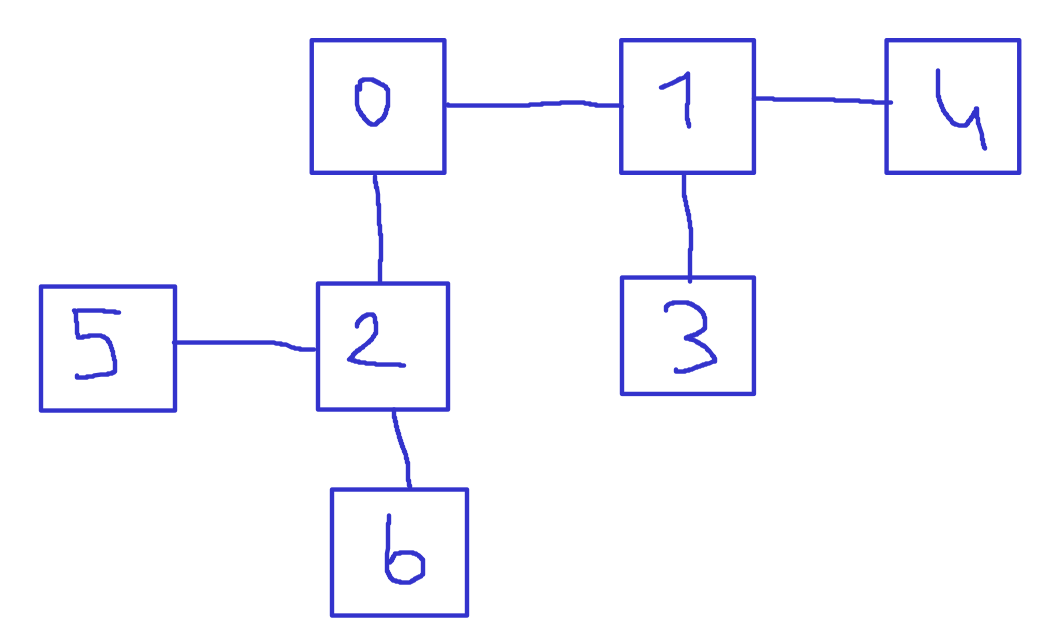
\includegraphics[width=0.5\textwidth]{images/bfs.png}
    \caption{}
\end{figure}

\begin{lstlisting}[language=Python]
from collections import deque

def breath_first_search(graph, start):
    visited = [False] * len(graph)
    queue = deque([start])
    visited[start] = True
    while queue:
        current_node = queue.popleft()
        print(current_node, end=" ")
        for neighbor in graph[current_node]:
            if not visited[neighbor]:
                queue.append(neighbor)
                visited[neighbor] = True


graph = {0: [1, 2], 1: [0, 3, 4], 2: [0, 5, 6],
         3: [1], 4: [1], 5: [2], 6: [2]}
breath_first_search(graph, start=1)
# 1 0 3 4 2 5 6 
\end{lstlisting}

\newpage

\subsection{Depth-First Search (DFS)}

Depth-First Search (DFS), bir graf ya da ağaç üzerindeki düğümleri derinlik öncelikli ziyaret eden bir arama algoritmasıdır. DFS, bir dalı tamamen keşfedene kadar derinlemesine iner, geri döner ve diğer dallara aynı işlemi uygular. Yani, her düğümün olabildiğince derinine inip keşfetmek temel stratejisidir. DFS, önce bir düğümden olabildiğince derine iner, bir yol tıkanırsa (yeni düğüm kalmazsa) geri dönerek diğer yolları keşfeder. Eğer graf sonluysa, DFS mutlaka bir çözüm bulur. Ancak, döngüler içeren sonsuz graflarda çözüm bulamayabilir. DFS en kısa yolu bulmayı garanti etmez, bu nedenle optimal değildir. Graf, $V$ düğüm ve $E$ kenardan oluşuyorsa, zaman karmaşıklığı $O(V + E)$'dir. Yani her düğüm bir kez ziyaret edilir ve her kenar bir kez işlenir.

\subsubsection{Python Kodu}

\begin{figure}[h]
    \centering
    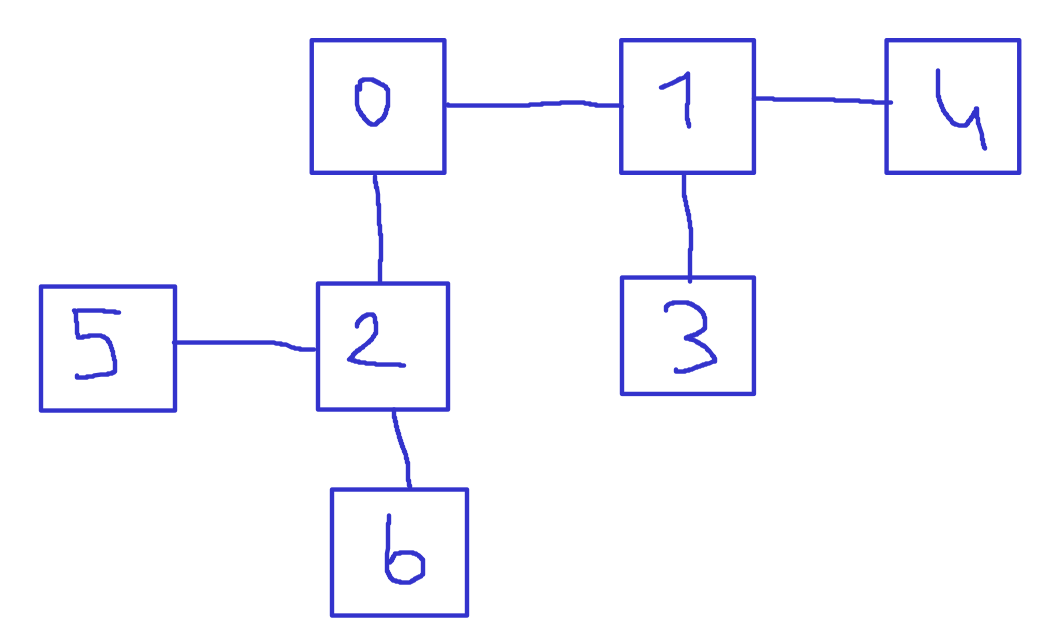
\includegraphics[width=0.5\textwidth]{images/dfs.png}
    \caption{}
\end{figure}

\begin{lstlisting}[language=Python]
def depth_first_search(graph, start):
    visited = [False] * len(graph)
    stack = [start]
    while stack:
        current_node = stack.pop()
        if not visited[current_node]:
            visited[current_node] = True
            print(current_node, end=" ")
            for neighbor in reversed(graph[current_node]):
                stack.append(neighbor)

graph = {0: [1, 2], 1: [0, 3, 4], 2: [0, 5, 6],
         3: [1], 4: [1], 5: [2], 6: [2]}
depth_first_search(graph, start=1)
# 1 0 2 5 6 3 4 
\end{lstlisting}

\newpage

\subsection{Uniform Cost Search (UCS)}

Uniform Cost Search (UCS), bir BFS türüdür, ancak farkı, kenar ağırlıklarını dikkate alarak en düşük maliyetli yolu bulmasıdır. UCS, her zaman en düşük maliyetli düğümü genişleterek hedefe ulaşmaya çalışır. UCS, her adımda en düşük maliyetli düğümü genişletir. Her kenarın ağırlığı (maliyeti) varsa, BFS'den farklı olarak bu ağırlıkları hesaba katar. Eğer çözüm varsa, UCS onu mutlaka bulur. UCS, en düşük maliyetli çözümü bulur, yani optimaldir. Düğüm genişletme işlemi her zaman maliyeti en düşük düğümle yapılır, böylece en kısa yol garantilenir. UCS'in zaman karmaşıklığı, genişletilen düğümlerin sayısına bağlıdır. En kötü durumda, her düğüm genişletildiğinde maliyet kontrol edilir, bu da $O((V + E) \text{log}V)$'dir, burada $V$ düğüm sayısı ve $E$ kenar sayısıdır.

\subsubsection{Python Kodu}

\begin{figure}[h]
    \centering
    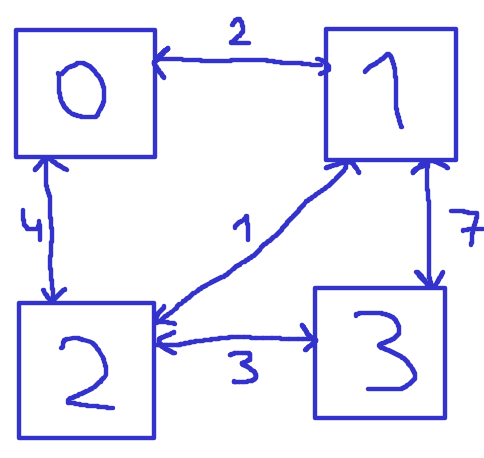
\includegraphics[width=0.5\textwidth]{images/ucs.png}
    \caption{}
\end{figure}

\begin{lstlisting}[language=Python]
import heapq

def uniform_cost_search(graph, start, goal):
    priority_queue = [(0, start)]
    visited = [False] * len(graph)
    cost_so_far = [float("inf")] * len(graph)
    cost_so_far[start] = 0
    while priority_queue:
        current_cost, current_node = heapq.heappop(priority_queue)
        if current_node == goal:
            return current_cost

        if visited[current_node]:
            continue

        visited[current_node] = True
        for neighbor, cost in graph[current_node]:
            new_cost = current_cost + cost
            if new_cost < cost_so_far[neighbor]:
                cost_so_far[neighbor] = new_cost
                heapq.heappush(priority_queue, (new_cost, neighbor))

    return float("inf")

graph = {0: [(1, 2), (2, 4)], 1: [(0, 2), (2, 1), (3, 7)], 
         2: [(0, 4), (1, 1), (3, 3)], 3: [(1, 7), (2, 3)]}
uniform_cost_search(graph, start=0, goal=3) # 6
\end{lstlisting}

\newpage

\subsection{Depth-Limited Search (DLS)}

Depth-Limited Search (DLS), bir çeşit DFS algoritmasıdır, ancak önceden belirlenmiş bir derinlik sınırı ile çalışır. Bu sınır, algoritmanın maksimum kaç derinlik seviyesine kadar arama yapacağını belirler. Eğer sınır aşılırsa, arama daha fazla derine gitmeden geri döner. DLS, DFS'in sonsuz derinliğe sahip grafiklerde veya ağaçlarda sonsuz döngüye girmesini engellemek için kullanılır. Eğer derinlik sınırı hedef düğümün seviyesinden küçükse, DLS hedefi bulamayabilir, bu nedenle tam değildir. Ancak, doğru sınır seçildiğinde tam olabilir. DLS, maliyet fonksiyonunu dikkate almaz, bu yüzden optimal değildir. Zaman karmaşıklığı, en kötü durumda $O(b^L)$'dir. Burada $b$ bir düğümün sahip olabileceği maksimum çocuk sayıdır ve $L$ derinlik sınırıdır.

\subsubsection{Python Kodu}

\begin{figure}[h]
    \centering
    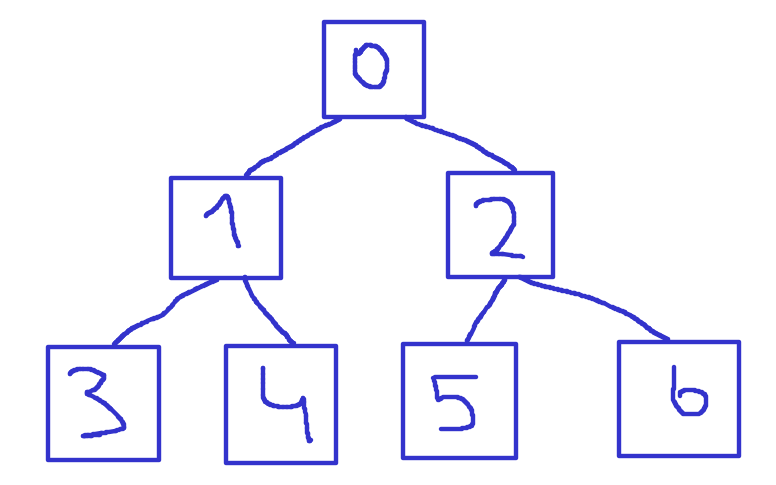
\includegraphics[width=0.5\textwidth]{images/dls.png}
    \caption{}
\end{figure}

\begin{lstlisting}[language=Python]
def reconstruct_path(stack, start, goal):
    path = [goal]
    while stack:
        node, _ = stack.pop()
        if node in path:
            break
        path.append(node)
    path.reverse()
    return path

def depth_limited_search(graph, start, goal, limit):
    stack = [(start, 0)]
    visited = set()

    while stack:
        node, depth = stack.pop()
        if node not in visited:
            visited.add(node)
            if node == goal:
                return reconstruct_path(stack, start, goal)
            if depth < limit:
                for neighbor in graph[node]:
                    stack.append((neighbor, depth + 1))
    return None

graph = {0: [1, 2], 1: [3, 4], 2: [5, 6], 
         3: [], 4: [], 5: [], 6: []}
depth_limited_search(graph, start=0, goal=6, limit=2)
# [1, 5, 6]
\end{lstlisting}

\newpage

\subsection{Iterative Deepening Depth-First Search (IDDFS)}

Iterative Deepening Depth-First Search (IDDFS), bir derinlik-sınırlı arama stratejisidir. Ancak bu stratejide, derinlik sınırı kademeli olarak artırılır. Yani, belirli bir derinlik sınırıyla başlar ve o sınırla bir DFS yapar. Eğer hedef bulunamazsa, sınır bir artırılır ve tekrar DFS yapılır. Bu işlem, hedef bulunana kadar devam eder. IDDFS, hem DFS hem de BFS yöntemlerinin avantajlarını birleştirir: DFS gibi az bellek kullanır. BFS gibi en kısa çözümü bulabilir (optimaldir) ve tamdır. IDDFS, sonlu bir ağaçta ya da grafikte hedef düğümün bulunduğu derinliğe kadar tüm seviyeleri sırasıyla araştırdığı için tamdır. IDDFS, en kısa çözüm yolunu bulur, bu yüzden BFS gibi optimaldir. Zaman karmaşıklığı, en kötü durumda $O(b^L)$'dir. Burada $b$ bir düğümün sahip olabileceği maksimum çocuk sayıdır ve $L$ derinlik sınırıdır.

\subsubsection{Python Kodu}

\begin{figure}[h]
    \centering
    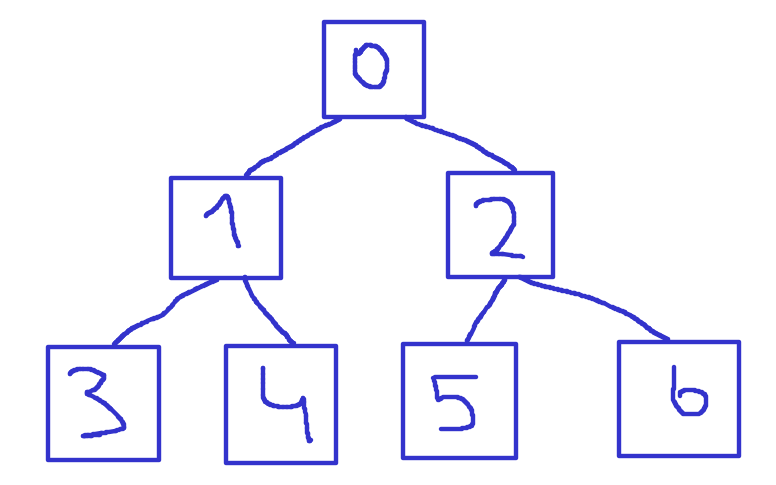
\includegraphics[width=0.5\textwidth]{images/iddfs.png}
    \caption{}
\end{figure}

\begin{lstlisting}[language=Python]
def iterative_deepening_dfs(graph, start, goal, limit):
    for depth in range(limit + 1):
        stack = [(start, 0)]
        visited = set()

        while stack:
            node, current_depth = stack.pop()
            if node not in visited:
                visited.add(node)
                if node == goal:
                    return depth
                if current_depth < depth:
                    for neighbor in graph[node]:
                        stack.append((neighbor, current_depth + 1))

    return None

graph = {0: [1, 2], 1: [3, 4], 2: [5, 6], 
         3: [], 4: [], 5: [], 6: []}
iterative_deepening_dfs(graph, start=0, goal=6, limit=3)
# 2
\end{lstlisting}

\newpage

\subsection{Bidirectional Search}

Bidirectional Search, hedef arama problemlerinde arama işlemini iki yönde aynı anda başlatan bir algoritmadır. Arama, hem başlangıç noktasından hedefe doğru ileri yönde yapılır, aynı zamanda hedeften başlangıç noktasına doğru geri yönde yapılır. Bidirectional Search, iki yönlü aramayı aynı anda çalıştırır. İleri yönde başlangıç düğümünden başlarken, geri yönde hedef düğümünden başlar. Her iki arama da genişlettikleri düğümleri birer veri yapısında tutar. Düğümlerden biri diğerinin genişlettiği düğümlerle kesiştiğinde, arama sona erer. Bu kesişim, çözümün bulunduğunu gösterir. Eğer bir çözüm varsa, bidirectional search kesinlikle bu çözümü bulur. Bu nedenle tamdır. İki yönlü arama, en kısa yolu bulur. Düğümler arasında aynı maliyete sahip yollar varsa optimal bir çözüme ulaşır. Zaman karmaşıklığı $O(b^{\frac{d}{2}})$'dir. Burada $b$ dallanma faktörü, $d$ hedef düğümün derinliğidir.

\subsubsection{Python Kodu}

\begin{figure}[h]
    \centering
    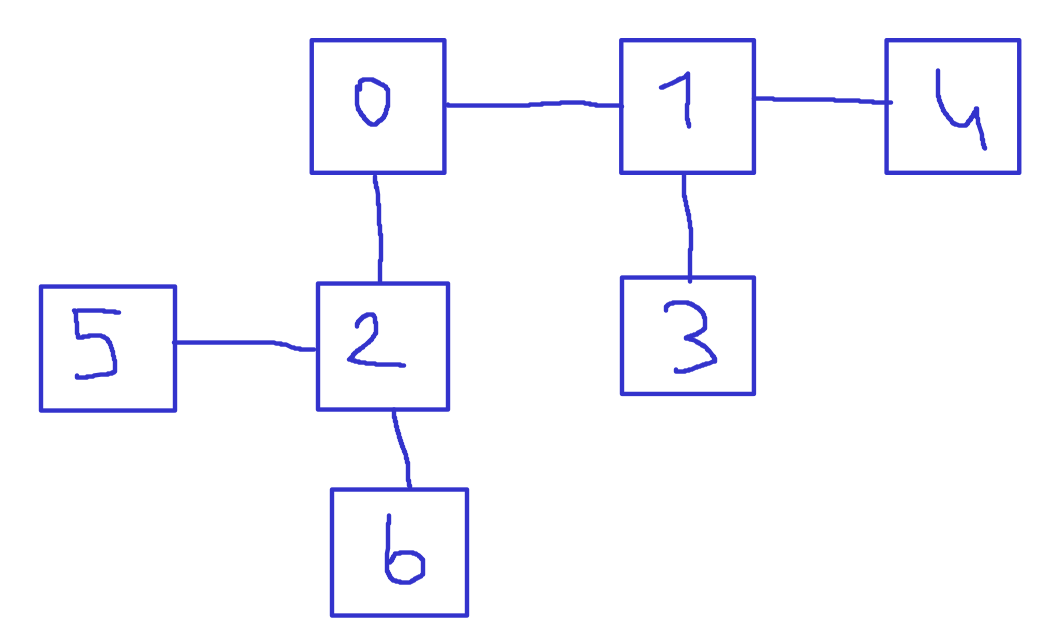
\includegraphics[width=0.5\textwidth]{images/bidirectional.png}
    \caption{}
\end{figure}

\begin{lstlisting}[language=Python]
from collections import deque

def bidirectional_search(graph, start, goal):
    start_queue = deque([start])
    goal_queue = deque([goal])
    start_visited = {start}
    goal_visited = {goal}

    while start_queue and goal_queue:
        current_node = start_queue.popleft()
        for neighbor in graph[current_node]:
            if neighbor in goal_visited:
                return True
            if neighbor not in start_visited:
                start_visited.add(neighbor)
                start_queue.append(neighbor)

        current_node = goal_queue.popleft()
        for neighbor in graph[current_node]:
            if neighbor in start_visited:
                return True
            if neighbor not in goal_visited:
                goal_visited.add(neighbor)
                goal_queue.append(neighbor)

    return False

graph = {0: [1, 2], 1: [0, 3, 4], 2: [0, 5, 6],
         3: [1], 4: [1], 5: [2], 6: [2]}
bidirectional_search(graph, start=0, goal=6)
# True
\end{lstlisting}

\newpage

\subsection{Best First Search}

Best First Search, her adımda en iyi görünen (en az maliyetli veya hedefe en yakın) düğümü genişletir. Bu seçim için bir heuristic (sezgisel) kullanılır. Sezgisel, düğümlerin hedefe ne kadar yakın olduğunu tahmin eden bir fonksiyondur ve algoritma her adımda bu tahmini en küçük olan düğümü genişletir. Sezgisel bir fonksiyonla düğümlerin hedefe yakınlığı tahmin edilerek seçim yapılır. Zaman karmaşıklığı $O(b^d)$'dir. Burada $b$ dallanma faktörü, $d$ hedef düğümün derinliğidir.

\subsubsection{Python Kodu}

\begin{figure}[h]
    \centering
    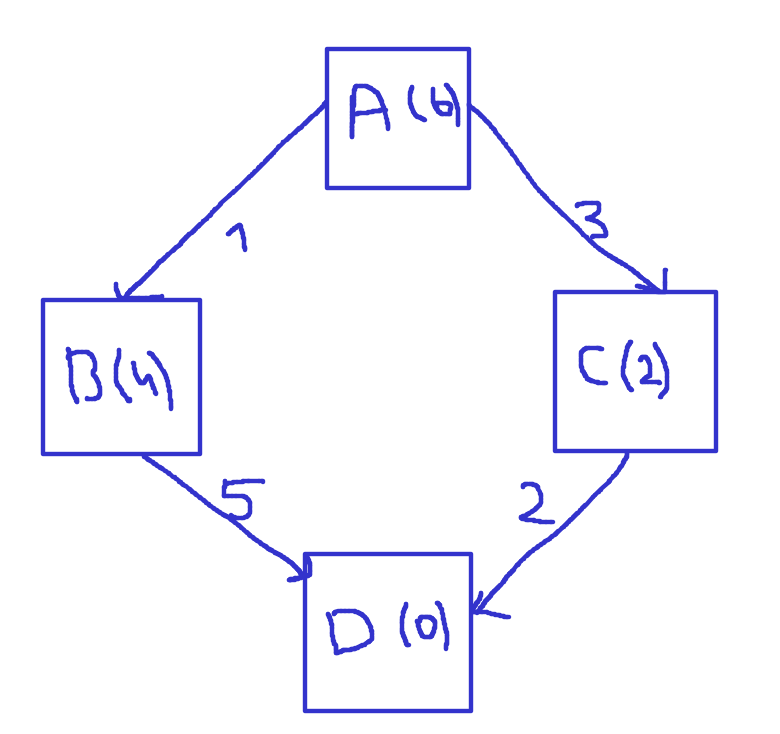
\includegraphics[width=0.5\textwidth]{images/best_first_search.png}
    \caption{}
\end{figure}

\begin{lstlisting}[language=Python]
import heapq

class Node:
    def __init__(self, name, heuristic):
        self.name = name
        self.heuristic = heuristic
        self.neighbors = []

    def add_neighbor(self, neighbor, cost):
        self.neighbors.append((neighbor, cost))

    def __lt__(self, other):
        return self.heuristic < other.heuristic

def best_first_search(start, goal):
    open_list = []
    heapq.heappush(open_list, start)
    visited = set()
    while open_list:
        current_node = heapq.heappop(open_list)
        if current_node.name == goal.name:
            return True
        
        visited.add(current_node)
        for neighbor, cost in current_node.neighbors:
            if neighbor not in visited:
                heapq.heappush(open_list, neighbor)
    
    return False

A = Node("A", 6)
B = Node("B", 4)
C = Node("C", 2)
D = Node("D", 0)
A.add_neighbor(B, 1)
A.add_neighbor(C, 3)
B.add_neighbor(D, 5)
C.add_neighbor(D, 2)
best_first_search(start=A, goal=D)
# True
\end{lstlisting}

\newpage

\subsection{A* Search}
A* Search, graf tabanlı problemlerde en kısa yolu bulmak için kullanılan güçlü bir informed search (bilgilendirilmiş arama) algoritmasıdır. Bu algoritma, hem en kısa yolu bulmayı hem de arama sürecini hızlandırmayı amaçlar. A* Search, iki temel bileşen kullanarak düğümlerin genişletilmesini yönetir:

\begin{itemize}
    \item $g(n)$: Başlangıç düğümünden $n$ düğümüne kadar olan maliyet (gerçek maliyet).
    \item $h(n)$: $n$ düğümünden hedefe olan tahmini maliyet (heuristic).
\end{itemize}

A* Search, her adımda düğümleri $f(n) = g(n) + h(n)$ maliyetine göre genişletir. Bu, algoritmanın her adımda hedefe en kısa yoldan gitmesini sağlar. A* Search, uygun bir heuristic kullanıldığında her zaman hedefi bulur, yani tamdır. A* algoritması, eğer heuristic tutarlı (consistent) ya da aşağılayıcı (admissible) ise en kısa yolu bulur. Aşağılayıcı heuristic, hiçbir zaman gerçek maliyeti aşmaz. Zaman karmaşıklığı, en kötü durumda $O(b^d)$'dir. Burada $b$ dallanma faktörü, $d$ hedef düğümün derinliğidir.

\subsubsection{Python Kodu}

\begin{figure}[h]
    \centering
    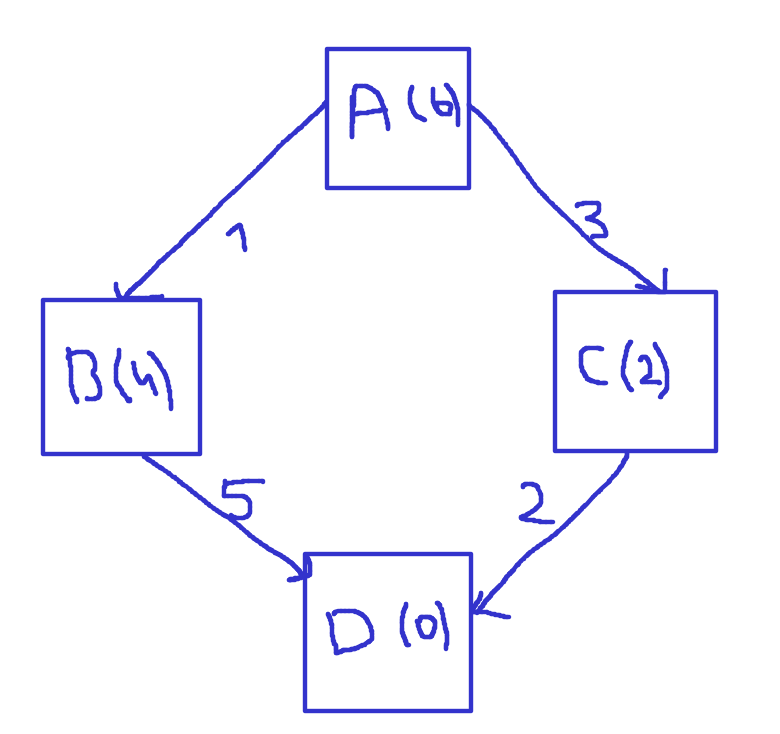
\includegraphics[width=0.5\textwidth]{images/a_start_search.png}
    \caption{}
\end{figure}

\begin{lstlisting}[language=Python]
class Node:
    def __init__(self, name, heuristic):
        self.name = name
        self.heuristic = heuristic
        self.neighbors = []

    def add_neighbor(self, neighbor, cost):
        self.neighbors.append((neighbor, cost))

    def __lt__(self, other):
        return self.heuristic < other.heuristic

def a_star_search(start, goal):
    g_values = {start: 0}
    open_list = [(start, start.heuristic)]
    visited = set()
    while open_list:
        current_node, _ = min(open_list, key=lambda x: x[1])
        open_list.remove((current_node, _))
        if current_node.name == goal.name:
            return True

        visited.add(current_node)
        for neighbor, cost in current_node.neighbors:
            if neighbor in visited:
                continue 

            new_g = g_values[current_node] + cost
            if neighbor not in g_values or new_g < g_values[neighbor]:
                g_values[neighbor] = new_g
                f_value = new_g + neighbor.heuristic
                open_list.append((neighbor, f_value))

    return False

A = Node("A", 6)
B = Node("B", 4)
C = Node("C", 2)
D = Node("D", 0)
A.add_neighbor(B, 1)
A.add_neighbor(C, 3)
B.add_neighbor(D, 5)
C.add_neighbor(D, 2)
a_star_search(start=A, goal=D)
# True
\end{lstlisting}

\newpage

\subsection{Dijsktra's Algorithm}

Dijkstra'nın algoritması, bir kaynaktan bir hedefe veya bir kaynaktan diğer tüm düğümlere en kısa yolları bulan bir greedy (açgözlü) algoritmadır. Yönlü ve pozitif ağırlıklı grafiklerde kullanılır. Temel amacı, bir başlangıç düğümünden diğer düğümlere en kısa yolu bulmaktır. Algoritma sadece pozitif ağırlıklı kenarları olan grafiklerde çalışır. Negatif ağırlıklar için kullanılmaz (Bellman-Ford algoritması negatif ağırlıklar için daha uygundur). Her adımda, en kısa yolu keşfetmek için açgözlü bir seçim yapılır. Yani, şu ana kadar bulunan en kısa mesafeli düğüm seçilir ve genişletilir.

\begin{enumerate}
    \item Kaynak düğümün başlangıç mesafesini sıfır yapılır ve diğer tüm düğümler için mesafeleri sonsuz olarak ayarlanır.
    \item Her düğüm için en kısa mesafe güncellenir ve en kısa mesafeye sahip düğümü seçilerek ilerlenir.
    \item Seçilen düğümden komşu düğümlere giden yolların maliyeti güncellenir.
    \item Tüm düğümler ziyaret edilene kadar bu işlemi tekrarlanır.
\end{enumerate}

\newpage

\subsection{Bellman-Ford Algorithm}

En kısa yolları bulmada kullanılır ve negatif ağırlıkların olduğu durumlarda tercih edilir. Bu algoritma, negatif ağırlıklı döngüleri de algılayabilir, bu da Dijkstra'nın algoritmasından önemli bir farktır. Ancak, Dijkstra algoritmasından daha yavaştır. ellman-Ford algoritması, negatif ağırlıklı kenarları olan grafikleri işleyebilir ve bu grafikleri doğru bir şekilde çalıştırabilir.  Grafikte negatif ağırlıklı döngüler (bir döngü boyunca toplam ağırlık negatif olan kenarlar) varsa, Bellman-Ford bunu tespit edebilir. Yönlendirilmiş veya yönlendirilmemiş grafiklerde çalışabilir.

\begin{enumerate}
    \item Başlangıç düğümünün mesafesi sıfır yapılır, diğer tüm düğümler için mesafeleri sonsuz olarak başlatılır.
    \item Tüm kenarlar $V - 1$ kez kontrol edilir. Her kontrol sırasında, hedef düğüme ulaşmanın daha kısa bir yolu varsa mesafe güncellenir.
    \item Eğer $V - 1$ iterasyondan sonra hala mesafeler güncelleniyorsa negatif döngü vardır.
\end{enumerate}

\newpage

\subsection{Floyd-Warshall Algorithm}

Floyd-Warshall algoritması, bir grafikteki tüm düğümler arasındaki en kısa yolları bulmak için kullanılan bir dinamik programlama algoritmasıdır. Bu algoritma, grafikteki her düğüm çiftinin arasındaki en kısa yolu bulur ve hem pozitif hem de negatif ağırlıklı kenarları destekler. Negatif ağırlıklı döngülerin olup olmadığını da tespit edebilir. Hem ağırlıklı hem de yönlendirilmiş grafiklerde çalışır.

\begin{enumerate}
    \item İlk başta, grafiğin uzaklık matrisi oluşturulur. Başlangıçta, her düğüm çiftinin arasındaki mesafe grafik üzerindeki kenar ağırlıkları ile başlatılır. Eğer düğümler arasında bir kenar yoksa mesafe sonsuz olarak başlatılır.
    \item Her düğüm, ara düğüm olarak kullanılarak, diğer düğüm çiftlerinin mesafeleri bu düğüm üzerinden geçip daha kısa hale gelip gelmediği kontrol edilir.
    \item Tüm düğümler için en kısa mesafeler hesaplandıktan sonra sonuç matrisi döndürülür.
\end{enumerate}

\newpage

\subsection{Kruskal's Algorithm}

Kruskal Algoritması, ağırlıklı ve bağlantılı bir grafikte Minimum Spanning Tree (MST) (minimum öbek ağaç) oluşturmak için kullanılan bir greedy algoritmadır. MST, bir grafikteki tüm düğümleri birbirine bağlayan minimum toplam ağırlıklı kenarlar kümesini temsil eder. Kruskal algoritması, ağacın minimum ağırlıklı kenarlarını seçerek, döngü oluşturmadan tüm düğümleri birbirine bağlayan bir alt grafik oluşturur. Algoritma, her adımda mevcut en düşük ağırlıklı kenarı seçerek ilerler. Her kenar eklendiğinde bir döngü oluşup oluşmadığı kontrol edilir. Döngü oluşursa kenar eklenmez. 

\begin{enumerate}
    \item Tüm kenarlar, ağırlıklarına göre artan şekilde sıralanır.
    \item Sırayla en küçük ağırlıklı kenarlar seçilir ve bu kenar eklendiğinde bir döngü oluşup oluşmadığı kontrol edilir.
    \item Döngü oluşumunu kontrol etmek için Union-Find veri yapısı kullanılır. Aynı kümeye ait olmayan iki düğüm birleştirilir.
    \item Tüm düğümler bağlantılı hale gelene veya seçilen kenar sayısı $V - 1$ olana kadar kenarlar eklenmeye devam edilir.
\end{enumerate}

\newpage

\subsection{Prim's Algorithm}

Prim’s Algoritması, ağırlıklı bir grafikte Minimum Spanning Tree (MST) (minimum öbek ağaç) oluşturmak için kullanılan bir greedy algoritmadır. Bu algoritma, belirli bir başlangıç düğümünden başlar ve her adımda, mevcut ağaca en yakın olan en düşük ağırlıklı kenarı seçerek ilerler. Bu sayede tüm düğümleri kapsayan bir ağ oluşturulur. Algoritma, belirli bir düğümden başlar ve her adımda ağaca en az ağırlıkla bağlanabilecek komşu düğümü seçer. Her adımda döngü oluşturulmadan yeni bir kenar eklenir. MST her adımda genişleyerek daha fazla düğüm kapsar. Her adımda en düşük ağırlıklı kenar seçilir.

\begin{enumerate}
    \item Rastgele bir düğüm seçilir.
    \item Her adımda mevcut ağaca en az ağırlıklı kenar eklenir.
    \item Yeni kenarın eklenmesi döngü oluşturmamalıdır.
    \item Tüm düğümler eklenene kadar işlem devam eder.
\end{enumerate}

\newpage

\subsection{Boruvka's Algorithm}

Boruvka'nın Algoritması, minimum öbek ağaç (Minimum Spanning Tree, MST) oluşturmak için kullanılan en eski algoritmalardan biridir. Bu algoritma, başlangıçta her düğümü kendi ağacı olarak kabul eder ve her adımda her ağaç için en düşük maliyetli kenarı ekleyerek büyüyen bir MST oluşturur. Borůvka'nın algoritması, küme tabanlı (component-based) bir yaklaşım kullanarak ilerler. Başlangıçta her düğüm bir küme oluşturur ve her adımda her küme, kendisine en düşük maliyetli kenarı ekleyerek başka bir kümeyle birleşir. Algoritma, her adımda birden fazla kenarı ekleyebildiği için paralel işlemeye uygundur. Her küme, kendisine en yakın düğümü bulur ve kenarı ekler. Bu süreç, tüm kümeler tek bir MST oluşturana kadar devam eder. Algoritma, her adımda mevcut kümeye en düşük maliyetli kenarı ekler.

\begin{enumerate}
    \item Her düğüm başlangıçta bağımsız bir küme olarak kabul edilir.
    \item Her adımda, her küme için en yakın düğümle olan en düşük maliyetli kenar seçilir.
    \item Bu kenarlar eklenerek kümeler birleşir.
    \item Tek bir küme (MST) oluşana kadar işlem devam eder.
\end{enumerate}

\newpage

\subsection{Kahn's Algorithm}

Kahn's Algorithm, yönlü bir grafiğin topolojik sıralamasını bulmak için kullanılan bir algoritmadır. Topolojik sıralama, bir DAG (Directed Acyclic Graph) üzerindeki düğümlerin sırasını bulur, bu sırada her kenar $(u, v)$ için $u$, $v$'den önce gelir. Yani, bir düğüme giden her yol önceki düğümden başlar. Bu algoritma, bir işin yapılma sırasını belirlemek veya bağımlılık sıralaması gereken durumlarda kullanılır. Yönlü, döngüsüz grafiğin düğümlerini, her düğümün yalnızca tüm bağımlılıkları çözüldükten sonra yerleştirilebileceği sıraya sokar. Algoritma, sadece döngüsüz yönlü grafiklerde uygulanabilir. Eğer grafik döngü içeriyorsa, topolojik sıralama yoktur. Her düğümün giriş derecesi (in-degree) hesaplanır, yani düğüme gelen kenarların sayısı. Giriş derecesi sıfır olan düğümler sıraya alınır.

\begin{enumerate}
    \item Tüm düğümlerin giriş dereceleri hesaplanır.
    \item Giriş derecesi sıfır olan düğümler bir sıraya eklenir.
    \item Bu düğümler sırayla işlenip grafikten çıkarılır. Grafikten çıkarılırken, bu düğümlerden giden kenarlar da kaldırılır ve bu kenarların hedef düğümlerinin giriş dereceleri azaltılır.
    \item Sıra boşalana ve tüm düğümler işlenene kadar devam edilir.
    \item Eğer işlenmeyen düğüm kalmımşsa, grafikte döngü vardır ve topolojik sıralam yapılmaz.
\end{enumerate}

\newpage

\subsection{Union-Find Algorithm}

Union-Find Algorithm (aynı zamanda Disjoint Set Union (DSU) veya Find-Union Algorithm olarak da bilinir), kümeler üzerinde etkili bir şekilde işlem yapmak için kullanılan bir veri yapısıdır. Bu algoritma, belirli kümelerde elemanların hangi kümeye ait olduğunu bulma (Find) ve iki kümenin birleşimini yapma (Union) işlemlerini hızlı bir şekilde gerçekleştirmek için kullanılır. Union-Find algoritması grafikte bağlantılı bileşenleri bulmak, Kruskal algoritması gibi minimum kovan ağacı (MST) algoritmalarında döngüleri tespit etmek ve çeşitli küme işlemlerini gerçekleştirmek için kullanılır.

\begin{enumerate}
    \item bir elemanın hangi kümeye ait olduğunu bulunur. Bu işlem, elemanın bağlı olduğu kök düğümü (temsilcisi) bulur. Tüm elemanlar bir kök düğüm tarafından temsil edilir.
    \item İki kümenin birleşimini gerçekleştirir. İki elemanın kök temsilcilerini bulur ve onları birleştirir.
    \item Find işlemi sırasında, her elemanı doğrudan kök düğümüne bağlamak için yol sıkıştırması yapılır. Bu, daha sonraki işlemleri hızlandırır.
    \item Union işlemi sırasında, daha küçük rütbeye sahip olan küme, daha büyük rütbeye sahip olan kümeye bağlanır. Bu, ağacın boyutunu küçük tutmak için kullanılır ve Find işlemini hızlandırır.
\end{enumerate}

\newpage

\subsection{Kosaraju's Algorithm}

Kosaraju's Algorithm, yönlü bir grafikte güçlü bağlı bileşenleri (Strongly Connected Components, SCC) bulmak için kullanılan etkili bir algoritmadır. Bir grafik içindeki bir bileşen, bileşen içindeki herhangi bir düğümden diğer herhangi bir düğüme ulaşılabilmesi durumunda "güçlü bağlı bileşen" olarak adlandırılır. Kosaraju'nun algoritması, iki derinlemesine arama (DFS) işlemiyle çalışır. 

\begin{enumerate}
    \item Grafikte tüm düğümler üzerinde DFS yaparak, düğümlerin bitiş zamanlarını hesaplar ve düğümleri bir yığın içine yerleştirir. Bu adımda grafiğin sadece düğümleri ve kenarları gezilir.
    \item Grafiğin transpozu (tersi) alınır. Bu adımda tüm kenarların yönü ters çevirilir.
    \item Yığından teker teker düğümleri alarak, ters grafikte DFS yapılır. Bu DFS işlemi sırasında her DFS çağrısı ile güçlü bağlı bileşen bulunur.
\end{enumerate}

\newpage

\subsection{Tarjan's Algorithm}

Tarjan's Algorithm, yönlü bir grafikte güçlü bağlı bileşenleri (Strongly Connected Components, SCC) bulmak için kullanılan bir başka etkili algoritmadır. Bu algoritma, DFS (Depth First Search) kullanarak tüm düğümleri ziyaret eder ve bir düğümün ait olduğu SCC'yi, o düğüm DFS'de ziyaret edilirken bulur. Tarjan’ın algoritması, düğümleri bir yığın kullanarak izler ve düğümün DFS’te keşfedilme zamanlarını ve geri dönülebilecek en düşük seviyeyi hesaplar. Algoritma, SCC'leri tespit etmek için yığın kullanır. Her düğüm, DFS sırasında geri dönebileceği en düşük bağlantı değerine sahiptir. Bu değer, düğümün hangi SCC'ye ait olduğunu belirlemek için kullanılır. Düşük bağlantı değeri ve keşif zamanı kullanılarak DFS sırasında geri çekilme yapılır.

\begin{enumerate}
    \item Algoritma, her düğümden bir DFS işlemi başlatarak tüm düğümleri ziyaret eder.
    \item Her düğüm için bir keşif zamanı atanır. Ayrıca her düğümün bağlı olduğu SCC'nin tespiti için düşük bağlantı değeri (low-link value) hesaplanır.
    \item Algoritma, DFS sırasında düğümleri bir yığında tutar. Eğer bir düğüm, kendi SCC'sinin kök düğümü ise, yığından bu SCC'yi çıkartarak güçlü bağlı bileşeni oluşturur.
\end{enumerate}

\newpage

\subsection{Ford-Fulkerson Algorithm}

Ford-Fulkerson Algoritması, bir akış ağındaki maksimum akışı bulmak için kullanılan bir algoritmadır. Bir kaynak düğümü (source) ile hedef düğüm (sink) arasında, kenar kapasitelerine saygı göstererek maksimum akışı bulmayı hedefler. Bu algoritma, artırılabilir yollar bularak bu yollar üzerinden akış değerlerini günceller ve sonucu elde eder. Algoritma, artan bir yol bulduğu sürece akışı artırmaya devam eder. Algoritma, her adımda orijinal grafiğin bir artık grafini oluşturur. Bu grafikte, mevcut kapasitelere göre akışlar hesaplanır.

\begin{enumerate}
    \item Tüm kenarlarda başlangıçta sıfır akış atanır.
    \item Kaynak düğümünden hedef düğüme giden ve artırılabilir kapasiteye sahip bir yol bulunur. Bu yol DFS veya BFS kullanılarak bulunabilir.
    \item Bu artırılabilir yol üzerindeki tüm kenarlar üzerinden maksimum artırılabilir kapasite kadar akış eklenir. Ayrıca, her artırma işlemiyle birlikte ters yöndeki akışlar da güncellenir.
    \item Artırılabilir bir yol bulunamadığında algoritma durur. Bulunan maksimum akış, bu noktada elde edilen toplam akış değeridir.
\end{enumerate}

\newpage

\subsection{Edmonds-Karp Algorithm}

Edmonds-Karp Algoritması, Ford-Fulkerson yönteminin bir genişletmesidir ve ağlarda maksimum akışı bulmak için kullanılır. Bu algoritma, artan yolları bulmak için BFS (Breadth-First Search) kullanır. BFS, her seferinde en kısa artan yolu bulmaya çalışarak algoritmanın çalışmasını garanti eder. Bu sayede, Ford-Fulkerson algoritmasının performansı iyileştirilir ve zaman karmaşıklığı daha belirgindir. 

\begin{enumerate}
    \item Kaynak düğümünden hedef düğüme sıfır akışla başlanır.
    \item BFS kullanarak kaynak düğümünden hedef düğüme giden artırılabilir bir yol bulunur.
    \item Bulunan yol üzerinden mümkün olan maksimum akış artırılır ve kenar kapasiteleri güncellenir. Ters yönlü akışlar da hesaba katılır.
    \item Artan bir yol bulunduğu sürece bu işlem tekrarlanır.
    \item Artan bir yol bulunamazsa, algoritma sona erer ve maksimum akış bulunmuş olur.
\end{enumerate}

\newpage

\subsection{Dinic's Algorithm}

Dinic's Algorithm, ağlarda maksimum akış bulmak için kullanılan bir algoritmadır ve Ford-Fulkerson metodunun bir uzantısıdır. Bu algoritma, BFS (Breadth-First Search) ve DFS (Depth-First Search) tekniklerini birleştirerek maksimum akışı daha hızlı bir şekilde bulur. Dinic’s algoritması, özellikle büyük ağlarda ve yüksek dereceli grafiklerde etkili bir şekilde çalışır. 

\begin{enumerate}
    \item Kaynak düğümünden başlayarak BFS kullanarak hedef düğüme ulaşabilecek artan yolları bulur ve katmanlı bir grafik oluşturur.
    \item Katmanlı grafikte DFS ile ilerleyerek artan yolları kullanır ve akışı artırır.
    \item Yeni bir katmanlı grafik oluşturup bu işlemi tekrarlayarak maksimum akışa ulaşılana kadar devam eder.
    \item BFS ile hedef düğüme ulaşamıyorsak, işlem tamamlanır ve maksimum akış bulunmuş olur.
\end{enumerate}

\newpage

\subsection{Push-Relabel Algorithm}

Push-Relabel Algoritması, maksimum akış problemini çözmek için kullanılan bir akış algoritmasıdır. Ağda maksimum akışı bulmak için yerel operasyonlar kullanır ve arttırma yollarını kullanmaz. Bu, Push-Relabel algoritmasını Ford-Fulkerson ve Dinic's gibi artan yol temelli algoritmalardan ayıran temel farktır. Fazla akışın olduğu bir düğümde, akış kenarlar üzerinden hedef düğümlere doğru "itilir" (push). Bir düğümün fazlası varsa, komşu düğümlere itebilir. Eğer bir düğümden itme yapılamıyorsa, o düğüm yeniden etiketlenir ve bir sonraki düğümün seviyesi artırılır. Kaynak düğümünden gelen akışlar, hedefine ulaşana kadar düğümler arasında dolaşır. Bir düğümde fazladan akış olursa, bu fazla akış diğer düğümlere gönderilir.

\begin{enumerate}
    \item Kaynak düğümden tüm komşu düğümlere maksimum kapasitede akış "itilir".
    \item Bir düğümde fazla akış varsa, akış komşu düğümlere doğru itilir. Eğer hedef düğüme giden bir yol varsa, bu yol üzerinden akış artırılır.
    \item Eğer akışın itilebileceği komşu düğüm yoksa, düğümün seviyesi artırılır.
    \item Bu işlemler tekrar edilerek tüm düğümler arasında maksimum akış hesaplanır.
\end{enumerate}

\newpage

\subsection{Greedy Coloring Algorithm}

Greedy Coloring Algoritması (Açgözlü Boyama Algoritması), bir grafın düğümlerini (nodelarını) boyarken, bitişik (komşu) düğümlerin aynı renkte olmamasını sağlamak için kullanılan basit ve sezgisel bir algoritmadır. Bu algoritmanın amacı, grafı minimum sayıda renk ile boyamaktır, ancak açgözlü bir strateji kullanıldığı için her zaman en az renk sayısını garanti etmez. Buna rağmen, pek çok pratik durumda iyi sonuçlar verebilir. Her düğüm sırasıyla ziyaret edilir ve o düğüm için mümkün olan en küçük renk atanır. Her düğüme renk atarken, sadece o anki komşu düğümler göz önünde bulundurulur. En kötü durumda, grafın düğüm derecesinden bir fazlası kadar renk kullanılabilir.

\begin{enumerate}
    \item Her düğüme renk atanmamış olarak başlanır.
    \item İlk düğümü alınır ve ona bir renk atanır.
    \item Her bir sonraki düğüm için, komşularının renkleri kontrol edilir ve kullanılmayan en küçük renkle o düğüm boyanır.
    \item Tüm düğümler boyanana kadar bu işlem tekrar edilir.
\end{enumerate}

\newpage

\subsection{Welsh-Powell Algorithm}

Welsh-Powell Algoritması, bir grafın düğümlerini renklendirme sorununu çözmek için kullanılan bir tür graph coloring (graf renklendirme) algoritmasıdır. Welsh-Powell algoritması, graf düğümlerini belirli bir sıralamaya göre renklendirir ve her bir düğüme, komşularıyla aynı renge sahip olmamasını sağlayacak şekilde en küçük uygun rengi atar. Düğümler sırayla en uygun renkle boyanır, yani mevcut düğüm için kullanılmayan en küçük renk atanır. Düğümler önce derecelerine göre (komşu sayısına göre) azalan bir sırayla sıralanır. En fazla komşusu olan düğüm önce boyanır.

\begin{enumerate}
    \item Grafın tüm düğümleri, derecelerine (komşu sayısı) göre azalan sırayla sıralanır.
    \item Her düğüm için, daha önce boyanmış komşuları ile aynı rengi almayan en küçük renk atanır.
    \item Tüm düğümler boyanana kadar işlem devam eder.
\end{enumerate}

\newpage